% IEEE standard conference template; to be used with:
%   spconf.sty  - LaTeX style file, and
%   IEEEbib.bst - IEEE bibliography style file.
% --------------------------------------------------------------------------

\documentclass[letterpaper]{article}

\usepackage 		 {amsmath	} % AMS mathematical facilities for LaTeX
\usepackage 		 {amssymb} % Amsfonts + few hundred additional mathematical symbols
\usepackage[english	]{babel	} 
\usepackage 		 {graphicx 	} % Enhanced support for graphics
\usepackage 		 {hyperref 	} % Extensive support for hypertext in LaTeX
\usepackage 		 {spconf 	} % Style file for Signal Processing Society Conferences

\usepackage{epstopdf	} % Convert EPS to 'encapsulated' PDF using GhostScript

\graphicspath{{figures/}} % Relative path to figures sources

\newcommand{\mypar}[1]{{\bf #1.}} % Bold paragraph titles

\title{Parallel Implementation of Breadth-First Search} % TODO: We need good descriptive title. This one is work version.

\name{Yauhen Klimiankou, Lukas Strebel, Stephanie Christ} 
\address{Department of Computer Science\\ ETH Z\"urich\\Z\"urich, Switzerland}

%TODO: ~5 figures (strong scaling + weak scaling on Intel + Xeon Phi and code snippet) + ~1 table (evaluation results).

% NOTE! Please, maintain the Pretty Print style of the document source code. Keep appropriate aligning and nesting, one sentence per line and separate paragraphs by empty line!

\begin{document}
	\maketitle

	\begin{abstract} % Roughtly half a column.
		% TODO: fill at the end of writing as a brief retelling of the whole paper content.
		 
		%%| Describe in concise words what you do, why you do it (not necessarily
		%%| in this order), and the main result. The abstract has to be
		%%| self-contained and readable for a person in the general area. You
		%%| should write the abstract last.
	\end{abstract}

	\section{Introduction}\label{sec:intro} % Roughtly page + TODO:~4 references.
		Graph is one of the most powerful and widely used abstract data type, because it is convenient for representation of wide range of real-world objects in computer applications.
		Most of the graph applications and appropriate algorithms involve graph traversals, during which knowledge's about graph is updated as each node and vertex become visited. 
		Depth-first search (DFS) and Breadth-first search (BFS) are two basic strategies for graph traversal and searching in graph.
		When the DFS starts graph traversal at the root and explores as far as possible along each branch before backtracking, BFS in contrast inspects all the neighboring nodes starting from the root and then for each of those neighbor nodes in turn, it inspects their neighbor nodes which were unvisited, and so on level by level.
		The set of nodes with the same distance from the root node is called a level in terms of BFS.
				
		BFS is one of the most basic graph algorithms and a foundation for wide range of more specific algorithms used for such tasks like finding of all nodes within one connected component of the graph, collection copying in garbage collection algorithms, finding of the shortest path between two specified nodes, testing a graph for bipartiteness, mesh numbering, computation of the maximum flow in a flow network etc.
		BFS is a first class algorithm commonly used for solving of different real-life and scientific problems on the systems represented by networks.
		Most notable examples of its industrial applications are navigation systems for finding of the shortest path between two specified destination points on the network of roads, finding of the shortest route to the specified host in the computer network or shortest route to the host with specified properties, web indexing performed by web crawlers used by web search engines to maintain they search database in the actual state, social interconnections investigation on the base of social networks.
		
		At this time the information technology industry experiencing a great shift introduced by mass migration to multi-core processors and emergence of many-core computer systems (up to 120/240 physical/logical cores in theory and up to 60/120 physical/logical cores in practice on Intel platform, and up to 64 physical cores on AMD platform) and coprocessors (computation accelerators) like Intel Xeon Phi (up to 61 physical cores).
		All this wide-spreading and emerging computer systems are examples of shared memory architectures (SMA).
		Wide dissemination of computer systems with shared memory architecture and trends indicating that the development of such systems is the main direction of the further performance improvement of computer systems on the one hand, and the widespread use of BFS for a wide range of applications makes actual the question about the most efficient and scalable variant of parallel version of BFS in the environment of such kind of systems.
		
		In this paper we describe an experimental study of different variants and approaches of parallel BFS based on the OpenMP for the SMA computer systems and design, implementation and  evaluation of the variant to which we finally came up as to the most promising.
		We refer to this variant as optimistic parallel BFS.
		According to our experimental results it significantly outperforms all other approaches in the environment of AMD SMA platform and Intel Xeon Phi accelerator.
		Our experiments and analysis of its results highlighted that the efficiency of BFS algorithm variants heavily depends on the properties of underlying environment (hardware platform, operating system, compiler) as well as on the properties of the graph to which it applied.   
		We conclude also that the cost of synchronization which is usually used for preserving consistency can be too high, but in some cases can be eliminated.
		
		It is important to note that the optimistic parallel BFS can't be considered as a universal optimal variant of BFS for the all kinds of the SMA computer systems.
		Instead it must be considered as a source of more general approach to the implementation of BFS for the environment of particular kind of SMA system.
		To achieve most optimal approach for particular computer system investigation of different variants of parallel BFS and most suitable optimizations must be done for the environment of system of interest, because our results tell us that the efficiency of BFS itself and optimizations used in it heavily depends on the target environment. 
	
	% \section{Experiments}\label{sec:expe} % Roughtly two pages - half a column. + 4 plots
	% \section{Discussion}\label{sec:disc} % Roughtly column. + ~1-2 references + 1 table
	% \section{Summary and Conclusion}\label{sec:suco} % Roughtly half a column.

	\section{Related work} \label{sec:rewo} % Roughtly column. + ~8 references.
		BFS is not an easy candidate for parallelization.
		It is inherently memory intensive and have pure spacial locality which introduces significant performance loss on the today computer systems with growing gap between CPU performance and memory performance and increasing memory latencies.
		As a result scalability of parallel version of BFS will be bound by the performance characteristics of the memory subsystem of the target computer system.. 
		Nevertheless intensive use of BFS in the wide range of the applications create high interest in the most efficient and scalable versions of parallel BFS.
		As a result a number of papers was published in this field. 
		
		Beamer et al.\cite{beamer2011searching} report a different algorithm to deal with the performance issues encountered when designing a BFS algorithm. 
		The proposed hybrid algorithm combines the usual top down approach with a new bottom up part. 
		In the bottom up part a level is processed by searching a parent for all unvisited vertices where a parent is only valid if it is a neighbour of the unvisited vertex. 
		This is advantageous for small-world graphs because it saves accesses and data processing when a large fraction of the vertices are in the frontier. 
		To get optimal results a hybrid algorithm is proposed where a heuristic switching criteria controls the use of top down or bottom up step depending on the size of the frontier and a predicted size of the next frontier. 
		Yasui et al.\cite{6691600} describe an implementation of such a hybrid algorithm for kronecker and R-MAT graphs as well as a detailed description of the heuristic switching parameters.
	
		Berrendorf\cite{Berrendorf:14} describes a technique to avoid atomic operations in a generalized scenario. 
		The scenario is given as an if-statement followed by some operations that change a state, where multiple threads might execute the predicate and execute the operations afterwards. 
		The operations need to change the state to the same value if executed multiple times otherwise there exists a race condition, i.e. the change of the distance of a visited vertex to the value of the level or the addition of a vertex to the next frontier. 
		The trade-off is that doing a BFS this way can result in additional work, since any unvisited vertex may get added multiple times.
		
		In our proposed technique we moves future at the way of avoiding atomic operations and intra-level synchronization at all.   
		The only synchronization point left in proposed algorithm is implicit barrier between processing of different levels of the graph.
		
		In addition to this we have compared a number of different approaches based on different synchronization primitives and techniques and load balancing strategies.
	
	\section{Design and implementation}\label{sec:deim} % Roughtly page + half a column. + 1 code snippet
		The goal of our efforts is to achieve most efficient and scalable algorithm of parallel BFS for Shared Memory Architectures. 

		\subsection{Possible directions of performance boosting}
			There are three main directions of performance boosting in the way of making BFS parallel.
			
			\textbf{Improvement of cache utilization improvement.}
			It is not a secret that due to the big gap between performance of CPU subsystem performance and memory subsystem performance of the modern computer systems and latencies of memory access makes performance of the algorithms highly sensitive to the provided CPU cache utilization. 
			Introduction of multicore computer systems made the problem even more complex because now we are forced to thinks about careful splitting of the active data set between all available processors to avoid cache misses introduced by cache lines flip-flopping. 
			Unfortunately in the case of the BFS we are forced to work with data set with inherently pure spatial locality. 
			Due to this this way of optimization was rejected.
			
			\textbf{Load balancing improvement.} 
			Goal of this approach is to achieve highest possible level of overall utilization of available processor elements via avoidance of the idle time of CPUs introduced by waiting for new job arriving.
			It is one of the promising approaches because classical approach to BFS parallelization relies on sequential graph level processing where each level is processed in parallel.
			As a result all CPU finished they work are forced to wait until the moment when current level processing will be accomplished by rest still busy processors.
			Nonetheless, this direction was rejected in favor of the synchronization avoidance. 
			
			\textbf{Avoidance of synchronization.}
			Synchronization is expensive but necessary component of the almost all parallel algorithms.
			Synchronization is expensive in both dimensions it usually takes a lot of CPU cycles in absolute numbers and reduce scalability.
			Our main design direction was figure out of the most cheap scheme of synchronization which will still provide consistency.
			Ideally we would like to eliminate synchronization at all.
			
		\subsection{Optimistic BFS algorithm design}
			Proposed algorithm was designed for the environment of the OpenMP and due to this employs data-parallelism approach. 
			It accepts two input parameters: graph description and index of the root node, where graph description is a list of lists in which each top-level list denotes of the graph vertexes and bottom level list enumerates all neighbors of the appropriate vertex thus denoting all edges connected to it and returns distance map for the specified root node.
			
			The core of proposed algorithm is classical. 
			It is level by level sequential top-down walking through the graph where on each iteration we discover all unvisited chills of the node presenting the current level.
			
			Algorithm utilize $4 \cdot number\_of\_the\_node$ bytes of memory allocated in 4 equal chunks:
			\begin{enumerate}
				\item x
			\end{enumerate}
			
	\section{Background: Breadth-first search}\label{sec:background}
	
	
	In this section we will give a brief overview over the idea of breadth-first search and its sequentiell asymptotic runtime cost and a short discussion of different graphs and graph properties. 
	
	
	\mypar{Breadth-first search}
		
	Breadth-first search (BFS) is a graph traversal algorithm which starts at a source and either travels until it finds a specific vertice or until it has explored all connected vertices. In the first step all vertices adjacent to the source are explored and stored in some data structure (called frontier or next) as well as marked as visited. In the second step the newly visited vertices become the new sources (called neighbours or current) from which the search continues by repeating this step. Doing a traversal in this way assures that all the nodes at the same distance to the source are explored on the same level before any vertices with greater distance can be explored. 
	
	The desired output of a BFS can differ depending on where it is applied. For example with minimal modifications BFS can deliever a predecessor map, where every vertex points to only one parent, or a distance map, where the distance to the source for every vertex is saved. Since the predecessor map is not necessarily unique, we choose to return a distance map as our output to make verification of correctness simpler.  
	
	The sequential version of a BFS can be implemented using a single queue and has a theoretical asymptotic runtime of $\mathcal{O}(\left|V\right|+\left|E\right|)$ where $\left|V\right|$ is the number of vertices and $\left|E\right|$ is the number of edges of the connected graph.
	
	
	\mypar{Graphs}
	
	
	
	% TODO
	% hybrid: doing topdown or bottum up, depending on heuristic switch. uses 1x OMP critical section in topdown part and localneighbourhoods + prefix sum to add them together at each level in the bottom up part. Idea from paper by Yasui et al
	% nonlevel: using 1xCAS to check visited and  1xOMP critical for the distance update (needs to see if unvisited or visited from further away), frontier is a single queue. if a thread finishes with his part he waits for the others to finish (no loadbalancing). Idea from talking with Timo.
	% nonlevel with work stealing. Idea is for threads that are finished with their part to steal work from a randomly choosen other thread. Only works with too much synchronization (slow) at the moment. Idea from talking with Timo.
	
	\section{Your Proposed Method}\label{sec:yourmethod}
	
	%Now comes the ``beef'' of the report, where you explain what you
	%did. Again, organize it in paragraphs with titles. As in every section
	%you start with a very brief overview of the section.
	%
	%In this section, structure is very important so one can follow the technical content.
	%
	%Mention and cite any external resources that you used including libraries or other code.
	
	We implemented many different algorithms and multiple variants for most of them. They return a distance map from one source vertex to all reachable vertices in the graph.
	
	All our implementations are based on OpenMP for synchronization.
	
	
	\mypar{Topdown}
	A lot of our approaches are based on a simple topdown algorithm. The idea is to do a level-synchronous traversal of the graph by keeping record of the vertices in the current as well as those in the next level (``frontier'' and ``neighbour'') in two data structures of the same type and setting the frontier to the current neighbours after each level. This leads to an implicit barrier, as the work done by the different threads has to be synchronized. We experimented with different data structures and synchronization methods.
	
	% naive
	% using 1x OMP critical section (check visited and add to frontier), frontier is a vector to allow easy dynamic splitting after each level (load balancing between threads). basically naive implementation
	The naive version of the topdown algorighm has a global standard vector for the frontier to allow easy dynamic splitting between the threads in each level. This balances the load between treads, however it has a significant overhead because it relies on a critical section (\verb+OMP critical+) for checking whether the vertices were already visited and inserting them into the neighbour data structure.
	
	% topdownCAS
	% using CAS (check visited) + OMP critical section (add to frontier), also vector frontier. Idea from paper by Berrendorf
	To improve the naive implementation, we used atomics, the built-in \verb+__sync_val_compare_and_swap+ (CAS) to atomically check whether a vertex was visited and set the correct distance. It also uses a local neighbourhood data structure (standard vector) to prevent needing a critical section. Only at the end of each level, a lock (\verb+omp_lock_t+) is used to combine the local neighbourhoods to a global one, which can then be distributed between the threads for the next level. This is an idea adapted from Berrendorf \cite{Berrendorf:14}.
	
	% topdown_ifCAS
	% same as topdownCAS but doing a nonatomic visited check before each CAS, Idea from paper by Berrendorf
	An extended version of the algorithm before first uses a non-atomic check if a vertex visited before each CAS.
	
	% topdown_nonatomic
	% doing the visited check nonatomic (adds additional work but no race condition), using localneighbourhood and OMP lock to add them to the global neighbourhood after a thread has looked at all neighbours from one node. Idea from paper by Berrendorf
	Also inspired by Berrendorf \cite{Berrendorf:14} is the idea to remove atomics alltogether. This results in a race condition where additional work for the next level is created, as some vertices might be added to the neighbours multiple times. However, expensive atomics are omitted, which results in a trade-off between the additional time from the added work and the faster runtime by leaving out the CAS. This algorithm still uses a local neighbourhood and a lock when combining them.
	
	% parallelbfs1
	% using 3x bool arrays for visited, looping over all nodes on each level, frontier is a mask
	Instead of using a standard vector for the frontier and the neighbour, one of our implementation relies on a bool array for all data structures (visited vertices, frontier, neighbour). This makes it possible to remove all critical sections, as the insertion of an element into a vector was what made them necessary in the first place. Similarly to the algorithm before, there might be additional work due to avoiding atomics. The downside of this implementation is that in each level, you have to loop through all the vertices, not just the current frontier, to be able to explore from there. Depending on the structure of the graph, this can be much more work.
	
	% TODO
	% tbb_parallelqueue
	% doing a topdown method using 1x OMP single for level synchronization and TBB concurrentqueue as a concurrent frontier
	
	% even_odd_parallelqueue
	% using only implicit OMP barrier for level synchronization. switching between two TBB parallelqueue frontiers
	
	
	
	
	\section{Experimental Results}\label{sec:exp}
	
	Here you evaluate your work using experiments. You start again with a
	very short summary of the section. The typical structure follows.
	
	\mypar{Experimental setup}
	%Specify the platform (processor, frequency, maybe OS, maybe cache sizes)
	%as well as the compiler, version, and flags used. If your work is about performance, 
	%I strongly recommend that you play with optimization flags and consider also icc for additional potential speedup.
	%
	%Then explain what kind of benchmarks you ran. The idea is to give enough information so the experiments are reproducible by somebody else on his or her code.
	%For sorting you would talk about the input sizes. For a tool that performs NUMA optimization, you would specify the programs you ran.
	We run experiments on three different platforms.
	
	The first platform is the EULER cluster which is operated by the HPC Group of ETH. We had access to one node with a 12-core Intel Xeon E5-2697v2 processors (2.7 GHz nominal, 3.0-3.5 GHz peak). It supports hyper-threading, so we ran our algorithms with up to 24 threads. On this platform, we used the gcc compiler with the -O2 flag.
	
	The next platform we ran our algorithms on is the Xeon Phi provided through the class.
	
	Lastly, we also used an AMD FX-8350 (4GHz x8, 8Gb, W2k3).
	
	% TODO
	\mypar{Results}
	Next divide the experiments into classes, one paragraph for each. In each class of experiments you typically pursue one questions that then is answered by a suitable plot or plots. For example, first you may want to investigate the performance behavior with changing input size, then how your code compares to external benchmarks.
	
	For some tips on benchmarking including how to create a decent viewgraph see pages 22--27 in
	
	
	
	{\bf Comments:}
	\begin{itemize}
	\item Create very readable, attractive plots (do 1 column, not 2 column plots
	for this report) with readable font size. However, the font size should also not be too large; typically it is smaller than the text font size.
	An example is in Fig.~\ref{fftperf} (of course you can have a different style).
	\item Every plot answers a question. You state this question and extract the
	answer from the plot in its discussion.
	\item Every plot should be referenced and discussed.
	\end{itemize}
	
	\begin{figure}\centering
	  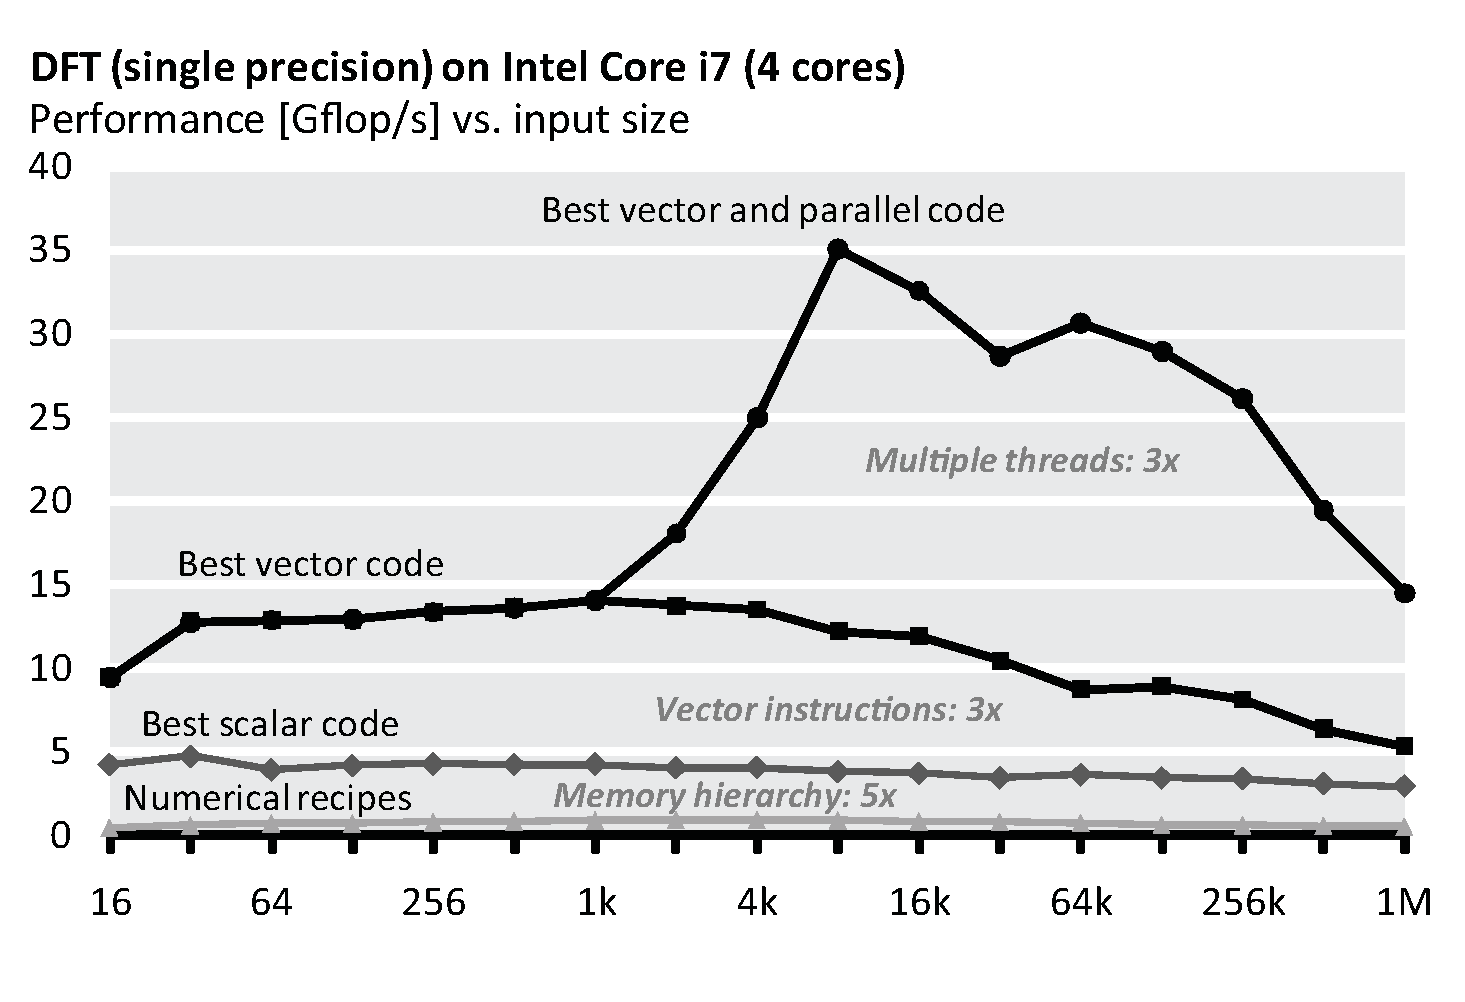
\includegraphics[scale=0.33]{dft-performance.eps}
	  \caption{Performance of four single precision implementations of the
	  discrete Fourier transform. The operations count is roughly the
	  same. The labels in this plot are maybe a little bit too small.\label{fftperf}}
	\end{figure}
	
	
	
	% TODO
	\section{Conclusions}
	
	Here you need to summarize what you did and why this is
	important. {\em Do not take the abstract} and put it in the past
	tense. Remember, now the reader has (hopefully) read the report, so it
	is a very different situation from the abstract. Try to highlight
	important results and say the things you really want to get across
	such as high-level statements (e.g., we believe that .... is the right
	approach to .... Even though we only considered x, the
	.... technique should be applicable ....) You can also formulate next
	steps if you want. Be brief. After the conclusions there are only the references.
	
	
	
	% TODO
	\section{Further comments}
	
	Here we provide some further tips.
	
	\mypar{Further general guidelines}
	
	\begin{itemize}
	\item For short papers, to save space, I use paragraph titles instead of
	subsections, as shown in the introduction.
	
	\item It is generally a good idea to break sections into such smaller
	units for readability and since it helps you to (visually) structure the story.
	
	\item The above section titles should be adapted to more precisely
	reflect what you do.
	
	\item Each section should be started with a very
	short summary of what the reader can expect in this section. Nothing
	more awkward as when the story starts and one does not know what the
	direction is or the goal.
	
	\item Make sure you define every acronym you use, no matter how
	convinced you are the reader knows it.
	
	\item Always spell-check before you submit (to us in this case).
	
	\item Be picky. When writing a paper you should always strive for very
	high quality. Many people may read it and the quality makes a big difference.
	In this class, the quality is part of the grade.
	
	\item Books helping you to write better:
	
	\item Conversion to pdf (latex users only): 
	
	dvips -o conference.ps -t letter -Ppdf -G0 conference.dvi
	
	and then
	
	ps2pdf conference.ps
	\end{itemize}
	
	\mypar{Graphics} For plots that are not images {\em never} generate the bitmap formats
	jpeg, gif, bmp, tif. Use eps, which means encapsulate postscript. It is
	scalable since it is a vector graphic description of your graph. E.g.,
	from Matlab, you can export to eps.
	
	The format pdf is also fine for plots (you need pdflatex then), but only if the plot was never before in the format 
	jpeg, gif, bmp, tif.


	\bibliographystyle 	{IEEEbib} % Roughtly column. (10-15 references).
	\bibliography 		{bibl_conf}
\end{document}

